% Slides for 2024-08-06
% To create a slide, use the following:



\begin{frame}{Segmentation using histogram equalization}
    \begin{minipage}{0.5\textwidth}
        \centering
        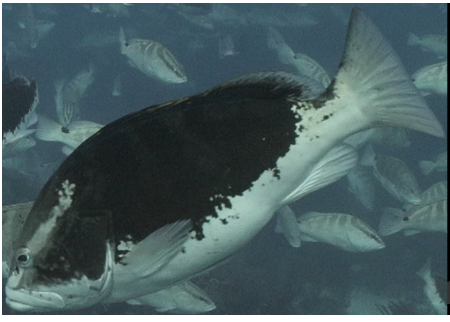
\includegraphics[height=0.7\textheight,keepaspectratio]{images/gm4-1.png}
    \end{minipage}%
    \begin{minipage}{0.5\textwidth}
        \centering
        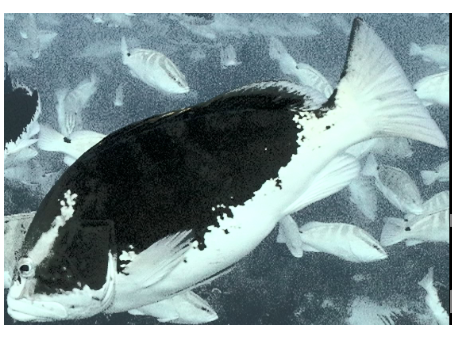
\includegraphics[height=0.7\textheight,keepaspectratio]{images/gm4-2.png}
    \end{minipage}
\end{frame}

\begin{frame}{Segmentation using histogram equalization}
    \begin{minipage}{0.5\textwidth}
        \centering
        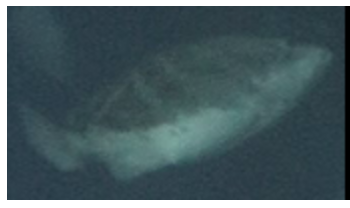
\includegraphics[width=\textwidth,keepaspectratio]{images/gm4-4.png}
    \end{minipage}%
    \begin{minipage}{0.5\textwidth}
        \centering
        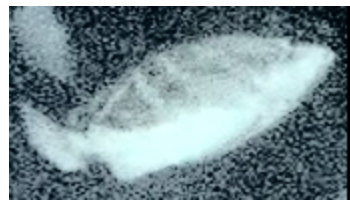
\includegraphics[width=\textwidth,keepaspectratio]{images/gm4-3.png}
    \end{minipage}
\end{frame}

\begin{frame}{Result comparision}
    \centering
      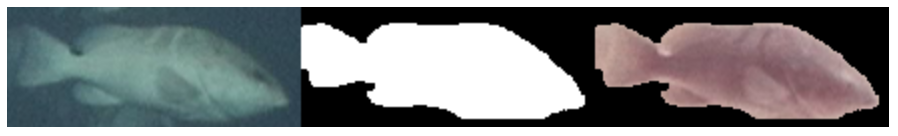
\includegraphics[height=0.7\textheight,width=0.7\textwidth,keepaspectratio]{images/gm4-5.png}
      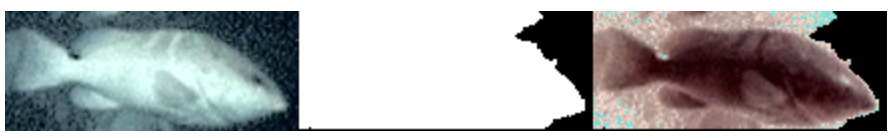
\includegraphics[height=0.7\textheight,width=0.7\textwidth,keepaspectratio]{images/gm4-6.png}

   
\end{frame}

\begin{frame}{Result comparision}
    \centering
      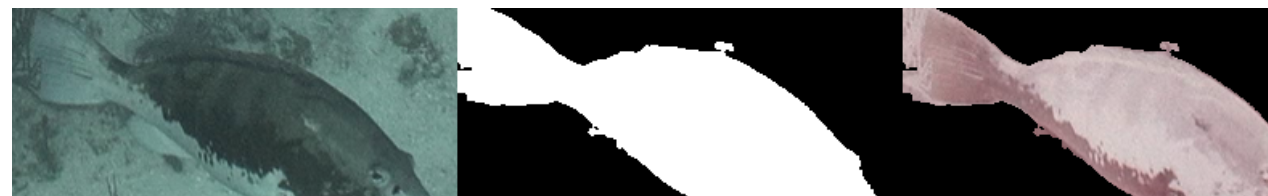
\includegraphics[height=0.7\textheight,width=0.7\textwidth,keepaspectratio]{images/gm4-7.png}
      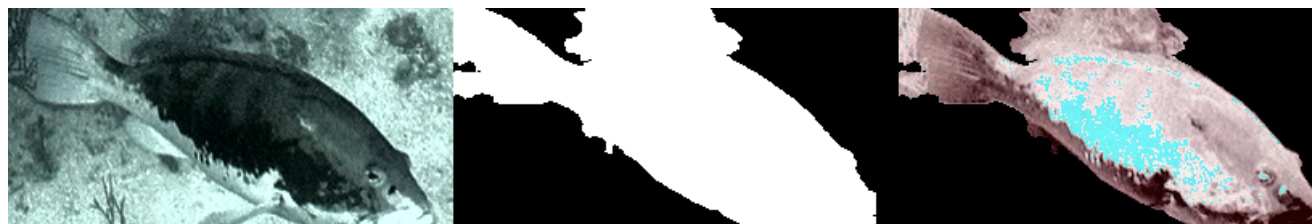
\includegraphics[height=0.7\textheight,width=0.7\textwidth,keepaspectratio]{images/gm4-8.png}
   
\end{frame}

\begin{frame}{Result comparision}
    \centering
      
\includegraphics[height=0.7\textheight,width=0.7\textwidth,keepaspectratio]{images/gm4-9.png}
      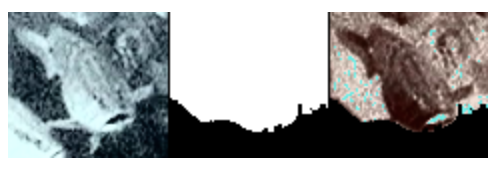
\includegraphics[height=0.7\textheight,width=0.7\textwidth,keepaspectratio]{images/gm4-10.png}
   
\end{frame}

\begin{frame}{Result comparision}
    \centering
      
\includegraphics[height=0.7\textheight,width=0.7\textwidth,keepaspectratio]{images/gm4-11.png}
      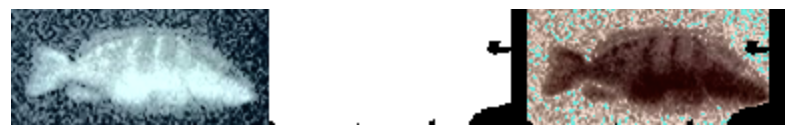
\includegraphics[height=0.7\textheight,width=0.7\textwidth,keepaspectratio]{images/gm4-12.png}
   
\end{frame}

\begin{frame}{Result comparision}
    \begin{itemize}
        \item Improved Recoginition: Improved the identification of previously unrecognized fish in the original images.
        \item Degraded Segmentation Quality: However, the introduction of noise adversely affected the overall quality of the segmentation results.
    \end{itemize}    
    
   
\end{frame}



\begin{frame}{Next step}
    \begin{itemize}
        \item Training yolo_v9 model using deep fish data and labeling party data
        \item Segment anything model 2 (SAM2)
    
   
\end{frame}








% To create a slide with a bullet list, use the following:
% \begin{frame}{TITLE}
%     \begin{itemize}
%         \item ITEM 1
%         \item ITEM 2
%     \end{itemize}    
% \end{frame}

% To create a slide with numbered list, use the following:
% \begin{frame}{TITLE}
%     \begin{enumerate}
%         \item ITEM 1
%         \item ITEM 2
%     \end{enumerate}
% \end{frame}

% To create a slide with a graphic:
% 1. Add the graphic to this folder (named picture.png)
% 2. Use the following:
% \begin{frame}{TITLE}
%     \centering
%     \includegraphics[height=0.7\textheight,width=0.7\textwidth,keepaspectratio]{picture.png}
% \end{frame}

% To create a slide with two columns, use the following:
% \begin{frame}{TITLE}
%     \begin{columns}
%         \begin{column}{0.5\textwidth}
%             COLUMN 1 BODY
%         \end{column}
%         \begin{column}{0.5\textwidth}
%             COLUMN 2 BODY
%         \end{column}
%     \end{columns}
% \end{frame}
